\documentclass[10pt]{beamer}

% ------------------------------------------------------------------------
% Carga de tu preámbulo personalizado (preamble.tex).
% Asegúrate de tenerlo en la misma carpeta para que \input funcione.
% ------------------------------------------------------------------------
\usetheme[progressbar=frametitle]{metropolis}
\usepackage{appendixnumberbeamer}
\usepackage{fancyvrb}
\usepackage{booktabs}
\usepackage[scale=2]{ccicons}
\usepackage{pgfplots}
\usepgfplotslibrary{dateplot}
\usepackage{type1cm}
\usepackage{lettrine}
\usepackage{ragged2e}
\usepackage{xspace}
\newcommand{\themename}{\textbf{\textsc{metropolis}}\xspace}
\usepackage{graphicx} % Allows including images
\usepackage{booktabs} % Allows the use of \toprule, \midrule and \bottomrule in tables
\usepackage[utf8]{inputenc} %solucion del problema de los acentos.
\usepackage{xcolor}
\definecolor{LightGray}{gray}{0.9}

\usepackage{minted}
\usemintedstyle{tango}
\newcommand{\mypyfile}[1]{\inputminted[linenos=true, fontsize=\footnotesize, frame=lines, framesep=5\fboxrule,framerule=1pt]{python}{#1}}

\setminted[python]{breaklines,frame=lines,framesep=2mm,baselinestretch=1.2,bgcolor=LightGray,linenos, fontsize=\footnotesize} % obeytabs=true, tabsize=2, showtabs=true}

%%%%%%%%%%%%%%%%%%%%%%%%%%%%%%%%%%%%%%%%%%%%%%%%%%%%%%%%%%%%%%%%%%%%%%%%%%%%%%%%%%%%%%
\setbeamercolor{progress bar}{fg=blue!50!black,bg=white!50!black}
\setbeamercolor{title separator}{fg=red!50!black,bg=white!50!black}
\setbeamercolor{frametitle}{fg=white!80!black,bg=red!50!black}
\title[PCFI161]{Programaci\'on para F\'isica y Astronom\'ia}
\subtitle{Departamento de Física.}

\newcommand{\myfront}{
\author[PCFI161]{Corodinadora: C Loyola \\ Profesoras/es C Loyola / C Femenías / Y Navarrete / C Ruiz}
\institute[UNAB]{Universidad Andrés Bello}
\date{Primer Semestre 2025}
}

\titlegraphic{%
  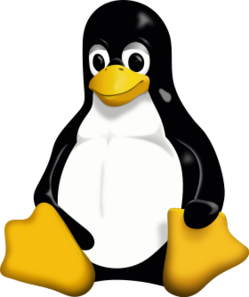
\includegraphics[width=.08\textwidth]{logo-tux.png}\hfill
  
\includegraphics[width=.3\textwidth]{logo-unab.png}\hfill
  
\includegraphics[width=.08\textwidth]{logo-python.png}
}

\makeatletter
\setbeamertemplate{title page}{
  \begin{minipage}[b][\paperheight]{\textwidth}
    \vfill%
    \ifx\inserttitle\@empty\else\usebeamertemplate*{title}\fi
    \ifx\insertsubtitle\@empty\else\usebeamertemplate*{subtitle}\fi
    \usebeamertemplate*{title separator}
    \ifx\beamer@shortauthor\@empty\else\usebeamertemplate*{author}\fi
    \ifx\insertdate\@empty\else\usebeamertemplate*{date}\fi
    \ifx\insertinstitute\@empty\else\usebeamertemplate*{institute}\fi
    \vfill
    \ifx\inserttitlegraphic\@empty\else\inserttitlegraphic\fi
    \vspace*{1cm}
  \end{minipage}
}
\makeatother


\makeatletter
\setlength{\metropolis@titleseparator@linewidth}{2pt}
\setlength{\metropolis@progressonsectionpage@linewidth}{2pt}
\setlength{\metropolis@progressinheadfoot@linewidth}{2pt}
\makeatother


\begin{document}

% ------------------------------------------------------------------------
% Portada de la Presentación
% ------------------------------------------------------------------------
\myfront{}

% ------------------------------------------------------------------------
% Slide 1: Título de la Sesión
% ------------------------------------------------------------------------
\begin{frame}
  \titlepage
  % Por ejemplo:
  % \title{Semana 8 - Sesión 2 (Sesión 16): Aplicaciones Prácticas y Evaluación Parcial en Clase}
\end{frame}

% ------------------------------------------------------------------------
% Slide 2: Índice / Tabla de Contenidos
% ------------------------------------------------------------------------
\begin{frame}
  \frametitle{Resumen - Semana 8, Sesión 2 (Sesión 16)}
  \tableofcontents
\end{frame}

% ------------------------------------------------------------------------
% Configuración de bloques
% ------------------------------------------------------------------------
\metroset{block=fill}

% ----------------------------------------------------------------------------------------
% SECCIÓN 1: Introducción y Repaso
% ----------------------------------------------------------------------------------------
\section{Introducción y Repaso}

% ------------------------------------------------------------------------
% Slide 3: Conexión con la Semana 7 y la Sesión 8.1
% ------------------------------------------------------------------------
\begin{frame}{Repaso y Contexto}
  \begin{itemize}
    \item \textbf{Semana 7} nos enfocamos en:
      \begin{itemize}
        \item Gráficos avanzados en Matplotlib (subplots, histogramas, 3D).
        \item Posible integración con pandas (archivos CSV), y animaciones/herramientas 3D.
      \end{itemize}
    \item \textbf{Semana 8, Sesión 1 (Sesión 15)}:
      \begin{itemize}
        \item Introducimos \textbf{POO} (clases, métodos, atributos) y combinamos con NumPy/pandas.
        \item Ejercicios de simulaciones o gestión de objetos en Python.
      \end{itemize}
    \item \textbf{Objetivo de hoy}: Aplicar y evaluar parte de lo visto en \textbf{Semana 7} (visualización y manipulación de datos), en un ejercicio integrador. Luego, tendremos discusión y retroalimentación.
  \end{itemize}
\end{frame}

% ------------------------------------------------------------------------
% Slide 4: Objetivos de la Sesión 16
% ------------------------------------------------------------------------
\begin{frame}{Objetivos de la Sesión 16}
  \begin{itemize}
    \item \textbf{Resolver} un \textbf{Problema a Evaluar} en grupos, enfocándonos en:
      \begin{itemize}
        \item Subplots avanzados, histogramas, 3D o datos tabulares (Semana 7).
        \item Generar o leer datos, procesarlos y graficarlos adecuadamente.
      \end{itemize}
    \item \textbf{Discutir} las soluciones y aclarar dudas posteriores.
    \item \textbf{Fomentar} la colaboración y la organización en un tiempo acotado (25-30 minutos).
  \end{itemize}
\end{frame}

% ----------------------------------------------------------------------------------------
% SECCIÓN 2: Problema a Evaluar
% ----------------------------------------------------------------------------------------
\section{Problema a Evaluar (Evaluación en Clase)}

% ------------------------------------------------------------------------
% Slide 5: Descripción del Problema
% ------------------------------------------------------------------------
\begin{frame}{Problema a Evaluar: Visualización Avanzada con Matplotlib}
  \textbf{Contexto} (Semana 7):
  \begin{itemize}
    \item Se practicaron \textbf{subplots múltiples}, \textbf{histogramas}, y \textbf{3D} con Matplotlib.
    \item Uso potencial de \texttt{pandas} para datos tabulares.
  \end{itemize}
  \vspace{0.3cm}

  \textbf{Tareas}:
  \begin{enumerate}
    \item Generar o leer un \textbf{DataFrame} con al menos 2 columnas cuantitativas (p.e., \texttt{x} e \texttt{y}) y 1 columna categórica (p.e., \texttt{categoria}).
      \begin{itemize}
        \item Puede ser \textbf{aleatorio} (\texttt{np.random}) o un archivo CSV sencillo.
      \end{itemize}
    \item Crear un \textbf{subplot con 2-3 paneles} (en una fila o columna):
      \begin{itemize}
        \item Panel 1: \textbf{Histogram} de la columna \texttt{x}.
        \item Panel 2: \textbf{Scatter plot} de \texttt{x} vs. \texttt{y}, coloreado por \texttt{categoria}.
        \item Panel 3 (opcional/bonus): un \textbf{plot 3D} si desean expandir, o un \textbf{boxplot} si lo prefieren.
      \end{itemize}
    \item Personalizar \textbf{etiquetas}, \textbf{títulos}, y \textbf{leyendas}.
  \end{enumerate}
\end{frame}

% ------------------------------------------------------------------------
% Slide 6: Instrucciones y Formato de Entrega
% ------------------------------------------------------------------------
\begin{frame}{Instrucciones para la Evaluación}
  \begin{itemize}
    \item Trabajar en \textbf{grupos de 2-3 estudiantes}.
    \item Crear un \textbf{notebook en Colab} (o un script local) llamado \texttt{Eval\_Semana8\_Apellidos.ipynb}.
    \item \textbf{Desarrollo} del problema:
      \begin{enumerate}
        \item Generar/leer datos (p. ej., \texttt{df = pd.DataFrame(...) o pd.read\_csv(...)}).
        \item Crear \textbf{subplots} y visualizar:
          \begin{itemize}
            \item Histograma de \texttt{x}.
            \item Scatter \texttt{x} vs \texttt{y}, color o marker según \texttt{categoria}.
            \item (Opcional) Tercer subplot: 3D simple, boxplot, o algo similar.
          \end{itemize}
        \item Etiquetar ejes, leyendas, título general si desean.
      \end{enumerate}
    \item Al finalizar (máximo \textbf{25-30 minutos}), \textbf{subir el archivo} a \textbf{CANVAS} (una entrega por grupo).
  \end{itemize}
\end{frame}

% ------------------------------------------------------------------------
% Slide 7: Pautas de Evaluación
% ------------------------------------------------------------------------
\begin{frame}{Pautas de Evaluación}
  \textbf{Se considerarán los siguientes criterios}:
  \begin{itemize}
    \item \textbf{Funcionalidad} (40\%): el código corre sin errores y se generan los subplots requeridos.
    \item \textbf{Uso apropiado de Matplotlib} (20\%): subplots correctos, buenas prácticas de rotulación.
    \item \textbf{Manejo de Datos} (20\%): DataFrame, lectura/generación de datos, coherencia de categorías, etc.
    \item \textbf{Organización/Comentarios} (20\%): claridad del notebook, explicaciones de cada paso.
  \end{itemize}
  \vspace{0.3cm}
  \textbf{Nota}: Se valoran detalles extra (filtros de datos, color maps, \texttt{plt.tight\_layout}, etc.).
\end{frame}

% ------------------------------------------------------------------------
% Slide 8: Tiempo de Desarrollo (25-30 min)
% ------------------------------------------------------------------------
\begin{frame}{Tiempo de Desarrollo}
  \begin{block}{}
    \huge{\textbf{Tienen 25-30 minutos para resolver y subir la solución a CANVAS.}}
  \end{block}
  \vspace{0.3cm}
  \textbf{Sugerencias}:
  \begin{itemize}
    \item Decidir rápido si generan datos (\texttt{np.random}) o usan un CSV existente.
    \item Asegurarse de \textbf{importar matplotlib} y \texttt{pandas} (si se usa).
    \item Revisar \textbf{leyendas}, \textbf{labels}, \textbf{titles} de cada subplot.
    \item \textbf{plt.tight\_layout()} para mejorar la presentación.
  \end{itemize}
\end{frame}

% ----------------------------------------------------------------------------------------
% SECCIÓN 3: Trabajo y Discusión Posterior
% ----------------------------------------------------------------------------------------
\section{Trabajo y Discusión}

% ------------------------------------------------------------------------
% Slide 9: Espacio de Resolución y Entrega
% ------------------------------------------------------------------------
\begin{frame}{Espacio de Resolución}
  \begin{itemize}
    \item \textbf{Pueden hablar en voz baja} para coordinar, cada grupo crea su notebook o script.
    \item Consultas breves en caso de bloqueos severos, pero intenten ser autónomos.
    \item Asegúrense de \textbf{probar la ejecución completa} antes de subir a CANVAS.
  \end{itemize}
\end{frame}

% ------------------------------------------------------------------------
% Slide 10: Cierre de la Evaluación
% ------------------------------------------------------------------------
\begin{frame}{Entrega Final}
  \begin{block}{Subida a CANVAS}
    \begin{itemize}
      \item Un integrante del grupo debe subir el \textbf{notebook .ipynb} (o .py) dentro del plazo (25-30 min).
      \item Revisen que estén todos los subplots requeridos.
      \item Comentar en Markdown o en el código el enfoque y los pasos.
    \end{itemize}
  \end{block}
  \vspace{0.3cm}
  \textbf{Tras la entrega}, discutiremos brevemente soluciones y dificultades encontradas.
\end{frame}

% ------------------------------------------------------------------------
% Slide 11: Discusión de Resultados
% ------------------------------------------------------------------------
\begin{frame}{Discusión Posterior}
  \begin{itemize}
    \item ¿Fue sencillo combinar \textbf{histograma} y \textbf{scatter} en subplots?
    \item ¿Cómo asignaron colores al \texttt{scatter} según la categoría? (p. ej. \texttt{c=...} o \texttt{hue=...} en Seaborn).
    \item ¿Dificultades con \textbf{figsize} o la disposición de subplots?
    \item ¿El tiempo de 25-30 min fue suficiente?
  \end{itemize}
\end{frame}

% ------------------------------------------------------------------------
% Slide 12: Resumen de la Evaluación
% ------------------------------------------------------------------------
\begin{frame}{Resumen de la Evaluación}
  \begin{itemize}
    \item Actividad integró:
      \begin{itemize}
        \item \textbf{Generación/lectura de datos} (DataFrame).
        \item Gráficas \textbf{subplots} avanzadas (hist, scatter, 3D o boxplot opcional).
        \item Personalización y estilos de Matplotlib (Semana 7).
      \end{itemize}
    \item Apunta a \textbf{manejo fluido} de Matplotlib para presentaciones de datos.
    \item Revisión más detallada y retroalimentación vendrá tras la clase.
  \end{itemize}
\end{frame}

% ----------------------------------------------------------------------------------------
% SECCIÓN 4: Cierre de la Sesión y Próximos Temas
% ----------------------------------------------------------------------------------------
\section{Cierre y Próximos Pasos}

% ------------------------------------------------------------------------
% Slide 13: Conclusiones de la Sesión 16
% ------------------------------------------------------------------------
\begin{frame}{Conclusiones de la Sesión 16}
  \begin{itemize}
    \item Ejecutamos un \textbf{problema evaluado} enfocado en \textbf{visualización avanzada} (subplots/hist/scatter) de la Semana 7.
    \item Observamos \textbf{estrategias} para leer/generar datos y graficarlos en Matplotlib.
    \item Discutimos \textbf{puntos complejos} (coloreo, layout, etiquetado).
    \item Continuamos la línea de integrar datos reales y presentarlos de forma clara.
  \end{itemize}
\end{frame}

% ------------------------------------------------------------------------
% Slide 14: Próxima Sesión
% ------------------------------------------------------------------------
\begin{frame}{Próximos Temas (Semana 9)}
  \begin{itemize}
    \item Avanzar con \textbf{POO} más complejo (herencia, polimorfismo) o \textbf{análisis de datos} más avanzado (estadísticas, merges).
    \item Revisar \textbf{retroalimentación} del problema actual en la siguiente clase.
    \item ¡Sigan practicando la personalización de subplots y la integración con \texttt{pandas}!
  \end{itemize}
\end{frame}

% ------------------------------------------------------------------------
% Slide 15: Recursos Adicionales
% ------------------------------------------------------------------------
\begin{frame}{Recursos Adicionales}
  \begin{itemize}
    \item \href{https://matplotlib.org/stable/gallery/index.html}{\textbf{Matplotlib Gallery}} - Inspírate con ejemplos.
    \item \href{https://pandas.pydata.org/}{\textbf{pandas Docs}} - para manipular DataFrames.
    \item \href{https://seaborn.pydata.org/}{\textbf{Seaborn}} - librería para gráficos estadísticos basados en Matplotlib (opcional).
  \end{itemize}
\end{frame}

% ------------------------------------------------------------------------
% Slide 16: Cierre de la Sesión
% ------------------------------------------------------------------------
\begin{frame}
  \Huge{\centerline{¡Buen trabajo y hasta la próxima sesión!}}
  \vspace{0.5cm}
  \normalsize
  \begin{itemize}
    \item Recuerden revisar notas y feedback en CANVAS.
    \item Cualquier duda, ¡pregúnten en foros o a sus compañeros!
  \end{itemize}
\end{frame}

\end{document}

